\documentclass[12pt, a4paper]{article}
\usepackage{graphicx} 
\usepackage{geometry}
\geometry{a4paper, margin=1in}
\usepackage{tikz}
\usetikzlibrary{calc}
\usepackage{hyperref} 
\usepackage{color}
\usepackage{array} % For centering content in table cells
\usepackage{lipsum} % For placeholder text

% Title, author, and date
\title{
    \vspace{-2cm}
    \Huge \textbf{\color{black!60} Software Tools and Technology}\\[0.5cm]
    
\includegraphics[width=0.3\linewidth]{Makaut.png}\\[0.5cm]
    \LARGE \textbf{\color{black} Lab Notebook}
}
\author{
    \vspace{1cm}
    \Large Group 05
}
\date{} % Leave empty to manually specify the date

\begin{document}
\maketitle
\pagenumbering{gobble}

% Border
\begin{tikzpicture}
    [remember picture, overlay]
    \draw[line width = 2pt, black] 
        ($(current page.north west) + (1cm,-1cm)$) 
        rectangle 
        ($(current page.south east) + (-1cm,1cm)$);
\end{tikzpicture}

\vspace{-1cm}
\begin{center}
\textbf{Repository Link:} \href{https://github.com/Nandini-Nath/LaTex_group-5}{\textcolor{blue!60}{https://github.com/Nandini-Nath/LaTex\_group-5}}
\end{center}

\vspace{1cm}

\centering
\bfseries{\underline{\Large \textcolor{blue!60}{Group Members}}}
\vspace{0.5cm}

\begin{flushleft}
\begin{enumerate}
    \item \textbf{Nandini Nath} \\
    Roll No: 30085323022 \\
    Department: BSc in IT (Cyber Security)
    
    \item \textbf{Subham Sanpui} \\
    Roll No: 30054623019 \\
    Department: BSc in IT (Artificial Intelligence)
    
    \item \textbf{Ankita Mondal} \\
    Roll No: 30001223053 \\
    Department: Bachelor of Computer Applications
    
    \item \textbf{Sourav Kundu} \\
    Roll No: 30001223076 \\
    Department: Bachelor of Computer Applications
    
    \item \textbf{Stuti Biswas} \\
    Roll No: 30059223049 \\
    Department: BSc in Forensic Science
\end{enumerate}
\end{flushleft}

\vspace{1cm}
\begin{center}
\textbf{Instructor:} \textcolor{blue!60}{Ayan Ghosh} \\
\vspace{0.3cm}
\textit{Date: \today}
\end{center}

\newpage
\begin{tikzpicture}
    [remember picture, overlay]
    \draw[line width = 2pt, black] 
        ($(current page.north west) + (1cm,-1cm)$) 
        rectangle 
        ($(current page.south east) + (-1cm,1cm)$);
\end{tikzpicture}
\vspace{-2cm}
% Index Table
\section*{\underline{\Huge\textbf{\textcolor{blue!60}{Index}}}}
\vspace{0.5cm}

\renewcommand{\arraystretch}{2} % Adjusts row height
\setlength{\tabcolsep}{0pt} % Adjusts column padding

\begin{tabular}{|>{\centering\arraybackslash}p{80pt}|>{\centering\arraybackslash}p{350pt}|}
\hline
\textbf{Serial No.} & \textbf{Questions} \\
\hline
1 & Introduction to GitHub and GitHub Desktop version installation \\\hline
2 & Building a C program for a calculator in the local repository,committing,and publishing it as a public repository \\\hline
3 & Converting a submit button to Chin Tapak Dum Dum \\\hline
% 4 & Placeholder for additional questions \\\hline
% 5 & Placeholder for conclusions \\\hline
% 6 & References used for this lab \\
% \hline
\end{tabular}

\newpage
\begin{tikzpicture}
    [remember picture, overlay]
    \draw[line width = 2pt, black] 
        ($(current page.north west) + (1cm,-1cm)$) 
        rectangle 
        ($(current page.south east) + (-1cm,1cm)$);
\end{tikzpicture}
\vspace{-2cm}
% Lab notebook entries
\section*{\Huge{\textcolor{blue!60}{Lab Notebook Entries}}}

% Each member writes their entry below
\subsection*{Entry by Nandini Nath}
\textit{Date: [\today]}\\

% Insert the image below the date and above the GitHub section
\begin{figure}[h!]
   \centering
    \includegraphics[width=0.5\linewidth]{Github_photo.png}
\end{figure}

\vspace{-1cm} % Adjust this value if you want more space between the image and the text below

\section*{\Huge{GitHub}}
\paragraph{GitHub is a web-based platform that allows developers to host, share, and collaborate on software projects. It provides a version control system powered by Git, enabling teams to track changes, manage code repositories, and work together seamlessly across different locations. GitHub supports collaborative development through features like pull requests, issues, and project boards, making it essential for open-source projects and professional software development. Additionally, it integrates with various development tools, enhancing productivity and streamlining the software development lifecycle.}

\subsection*{Installation}
\paragraph{Installing GitHub Desktop is a straightforward process that enhances your workflow by providing a user-friendly interface for managing repositories. To begin, download the installer from the [official GitHub Desktop website](https://desktop.github.com/) for your operating system—Windows or macOS. After downloading, run the installer and follow the on-screen instructions to complete the setup. Once installed, launch the application and sign in with your GitHub credentials, or create a new account if needed. GitHub Desktop simplifies the process of cloning repositories, making commits, and managing branches, making it an invaluable tool for developers of all skill levels. For Linux users, alternative methods like using Wine or other Git clients are available.}

\newpage
\begin{tikzpicture}
    [remember picture, overlay]
    \draw[line width = 2pt, black] 
        ($(current page.north west) + (1cm,-1cm)$) 
        rectangle 
        ($(current page.south east) + (-1cm,1cm)$);
\end{tikzpicture}
\vspace{-2cm}
\subsection*{Entry by Subham Sanpui}
\textit{Date: [\today]}\\
% Write your lab notebook entry here.

\newpage
\begin{tikzpicture}
    [remember picture, overlay]
    \draw[line width = 2pt, black] 
        ($(current page.north west) + (1cm,-1cm)$) 
        rectangle 
        ($(current page.south east) + (-1cm,1cm)$);
\end{tikzpicture}
\vspace{-2cm}
\subsection*{Entry by Ankita Mondal}
\textit{Date: [\today]}\\
% Write your lab notebook entry here.

\newpage
\begin{tikzpicture}
    [remember picture, overlay]
    \draw[line width = 2pt, black] 
        ($(current page.north west) + (1cm,-1cm)$) 
        rectangle 
        ($(current page.south east) + (-1cm,1cm)$);
\end{tikzpicture}
\vspace{-2cm}
\subsection*{Entry by Sourav Kundu}
\textit{Date: [\today]}\\
% Write your lab notebook entry here.

\newpage
\begin{tikzpicture}
    [remember picture, overlay]
    \draw[line width = 2pt, black] 
        ($(current page.north west) + (1cm,-1cm)$) 
        rectangle 
        ($(current page.south east) + (-1cm,1cm)$);
\end{tikzpicture}
\vspace{-2cm}
\subsection*{Entry by Stuti Biswas}
\textit{Date: [\today]}\\
% Write your lab notebook entry here.
\section*{\Huge{Git Assignment 3 : Branching and Merging}}

\paragraph{Objective:} Demonstrate proficiency in Git branching, merging, and conflict resolution.

\vspace{0.5cm}

% Manually resizing the images to fit within the page margins
% Screenshot 1
\begin{figure}[h!]
    \centering
    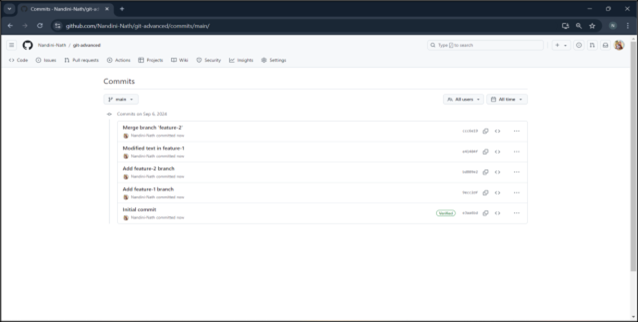
\includegraphics[width=0.8\linewidth]{LaTex_group_5/commit_history.png} % Adjusted width
     \hspace{4 cm}
    \caption{Screenshot of the GitHub repository showing the commit history.}
\end{figure}

% Screenshot 2 
\begin{figure}[h!]
    \centering
    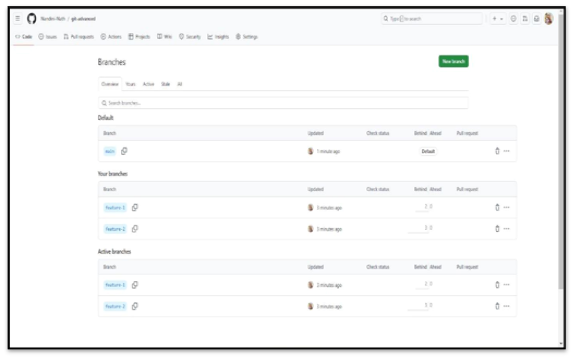
\includegraphics[width=0.8\linewidth]{LaTex_group_5/branching.png} % Adjusted width
     \hspace{4 cm}
    \caption{Screenshot of the GitHub repository showing the branching.}
\end{figure}
\newpage
\begin{tikzpicture}
    [remember picture, overlay]
    \draw[line width = 2pt, black] 
        ($(current page.north west) + (1cm,-1cm)$) 
        rectangle 
        ($(current page.south east) + (-1cm,1cm)$);
\end{tikzpicture}
\vspace{-1.5cm}
% Screenshot 3

\begin{figure}[h!]
    \centering
    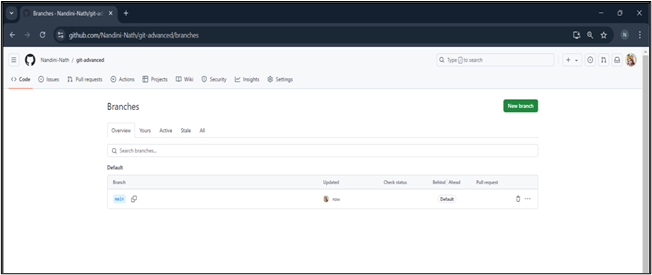
\includegraphics[width=0.8\linewidth]{LaTex_group_5/deleted_branches.png}
       \hspace{4 cm}
    \caption{Repository after deleting branches 'feature-1' and 'feature-2'.}
    \label{fig:enter-label}
\end{figure}
% Screenshot 4
\hspace{6 cm}
\begin{figure}[h!]
    \centering
    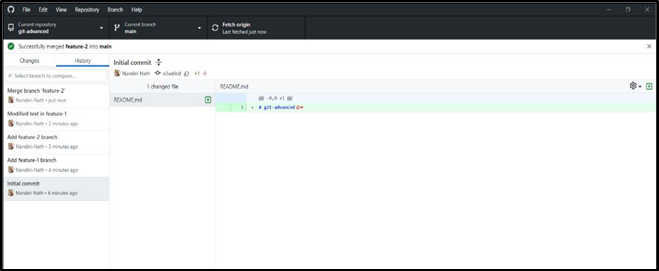
\includegraphics[width=0.8\linewidth]{LaTex_group_5/git_log.png} % Adjusted width
    \hspace{4 cm}
    \caption{Screenshot of the local machine showing the Git log.}
\end{figure}
\hspace{6 cm}
% Screenshot 5
\begin{figure}[h!]
    \centering
    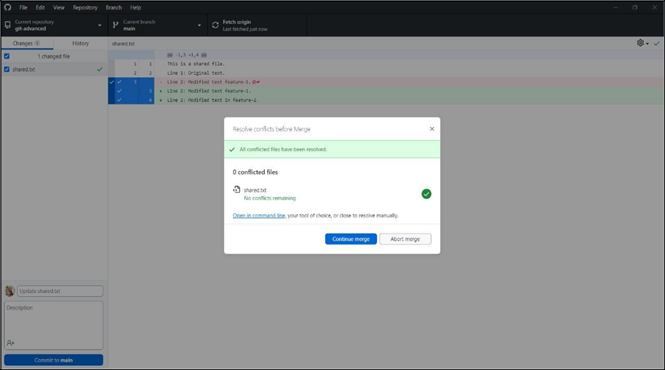
\includegraphics[width=0.8\linewidth]{LaTex_group_5/conflict_resolution.png} % Adjusted width
       \hspace{4 cm}
    \caption{Screenshot of the local machine showing conflict resolution.}
\end{figure}
\newpage
\begin{tikzpicture}
    [remember picture, overlay]
    \draw[line width = 2pt, black] 
        ($(current page.north west) + (1cm,-1cm)$) 
        rectangle 
        ($(current page.south east) + (-1cm,1cm)$);
\end{tikzpicture}
\vspace{-1.5cm}
\subsection*{\Huge{Write-Up: Experience with Git Branching and Merging}}
\hspace{1 cm}
\paragraph {This assignment focused on the use of Git branching and merging to manage features in a collaborative environment. After creating separate branches for feature-1 and feature-2, each was developed independently.
When merging feature-1 into the main branch, there were no conflicts. However, the merge of feature-2 caused a conflict in the shared.txt file. Conflict resolution was done manually, ensuring that the changes from both branches were retained.
The practical experience highlighted the importance of clear commit messages and Git’s branching capabilities for parallel development and conflict management.}

\end{document}
